%-*- coding: utf-8 -*-
\label{chap:estimation}

\paragraph{Notions :} échantillon aléatoire, estimateur, estimation, biais d'un
estimateur, convergence d'un estimateur, estimation par maximisation de la
vraisemblance, estimation de Bayes.
\paragraph{Objectifs pédagogiques :}
\begin{itemize}
\setlength{\itemsep}{3pt}
\item Choisir un estimateur, en particulier en déterminant des propriétés
  telles que son biais ou sa précision.
\item Proposer un estimateur, en particulier par maximisation de la
  vraisemblance.
\end{itemize}


\section{Inférence statistique}
Alors que la statistique descriptive se contente de \textit{décrire} une
population ou un échantillon de celle-ci, l'inférence statistique cherche à
tirer des conclusions sur une population à partir de l'étude d'un échantillon
de celle-ci. 

\section{Échantillonnage}
\label{ref:echantilonnage}

Lorsque la population à étudier est trop grande pour qu'il soit possible
d'observer chacun de ses individus, on étudie alors une partie seulement de la
population. Cette partie est appelée \textbf{échantillon}. On parle alors de
\textbf{sondage}, par opposition à un \textbf{recensement}, qui consiste à
étudier tous les individus d'une population.

\paragraph{Hypothèses de l'échantillonnage} Pour tirer parti d'un échantillon,
nous allons avoir besoin des hypothèses suivantes :
\begin{itemize}
\item La taille de la population est infinie ;
\item Les variables mesurées sur la population peuvent être considérées comme
  des variables aléatoires, dont les mesures sont des réalisations. Les lois de
  probabilité suivies par ces variables peuvent appartenir à une famille connue
  (e.g. loi gaussienne, loi de Poisson, etc.) ou être totalement
  inconnues. Dans le premier cas, on parlera de \textbf{statistique
    inférentielle paramétrique} ; dans le deuxième, de \textbf{statistique
    inférentielle non-paramétrique}.
\end{itemize}

\paragraph{Objectifs de la statistique inférentielle} La statistique
inférentielle a alors pour but d'\textbf{identifier les lois de probabilité de ces
  variables aléatoires.} Cela peut prendre les
formes suivantes :
\begin{itemize}
\item L'\textbf{estimation}, qui permet de déterminer les paramètres des lois (paramètre
  $p$ d'une loi de Bernoulli, indice et paramètre d'échelle d'une loi Gamma) ou
  certaines de leurs caractéristiques (espérance, variance, moments d'ordre
  supérieur, quartiles, etc.). C'est le sujet de ce chapitre.
\item Les \textbf{tests d'hypothèse}, qui permettent d'infirmer ou de confirmer des
  hypothèses faites sur ces lois, leurs paramètres ou leurs
  caractéristiques. Il s'agit par exemple de décider s'il est plausible que
  l'espérance d'une variable soit supérieure à une certaine valeur ; ou qu'une
  variable suive une loi normale. C'est le sujet du chapitre~\ref{chap:tests}. %Ce sujet dépasse le cadre de ce cours.
  
\end{itemize}

\paragraph{Échantillonnage aléatoire}
Dans la suite de ce chapitre, nous allons considérer que l'échantillon obtenu
par sondage est obtenu par \textbf{échantillonnage aléatoire simple} : on
prélève des individus dans la population au hasard, sans remise. Chaque
individu de la population a la même probabilité $1/N$ d'être prélevé, où $N$
est la taille de la population (on rappelle que $N \rightarrow \infty$) et les 
individus sont prélevés indépendamment les uns des autres.

\paragraph{Autres techniques d'échantillonnage} D'autres techniques
d'échantillonnage sont possibles, comme l'échantillonnage aléatoire
\textit{stratifié}, dans lequel la population est partitionnée en strates selon
une caractéristique (par exemple, par tranche d'âge), et l'échantillon est
obtenu en procédant à un échantillonnage aléatoire simple dans chacune des
strates. On obtient ainsi pour chaque strate un échantillon de taille
proportionnelle à la taille de la strate dans la population. En d'autres
termes, les individus n'ont pas tous la même probabilité d'être tirés :
celle-ci dépend de la taille de la strate à laquelle ils appartiennent.

\paragraph{Représentativité} Avant de tirer des conclusions d'un échantillon
aléatoire, il est important de s'assurer que celui-ci est représentatif de la
population étudiée. Par exemple, les premières études cliniques démontrant
l'efficacité de l'aspirine pour réduire le risque d'infarctus du myocarde chez
les patients à risque portaient sur des échantillons composés principalement
d'hommes ; ce n'est que bien plus tard que la communauté médicale a réalisé que
l'efficacité est bien moindre chez les femmes.

\paragraph{Échantillon aléatoire et échantillon} Deux échantillons $(x_1, x_2, \dots, x_n)$ et
$(x^\prime_1, x^\prime_2, \dots, x^\prime_n)$ de tailles identiques $n$ de la
même population seront donc différents. On modélise cette variabilité en
considérant que les individus $x_i$ et $x^\prime_i$ sont la réalisation
d'une même variable aléatoire $X_i.$ $(X_1, X_2, \dots, X_n)$ est un vecteur
aléatoire dont les composantes sont indépendantes et identiquement
distribuées (iid).
\begin{itemize}
\item $(X_1, X_2, \dots, X_n)$ est appelé \textbf{échantillon aléatoire} ;
\item $(x_1, x_2, \dots, x_n)$ et $(x^\prime_1, x^\prime_2, \dots, x^\prime_n)$
  sont deux échantillons, c'est-à-dire deux \textit{réalisations} de cet
  échantillon aléatoire.
\end{itemize}

Un indicateur statistique de l'échantillon est alors la réalisation d'une
variable aléatoire fonction de l'échantillon aléatoire.

\begin{exemple} La moyenne d'un échantillon,
$\bar{x} = \frac1n \sum_{i=1}^n x_i,$ est la réalisation d'une variable
aléatoire $M_n$ définie par
\[
  M_n = \frac1n \sum_{i=1}^n X_i,
\]
qui est une fonction de l'échantillon aléatoire $(X_1, X_2, \dots, X_n)$.
\end{exemple}

\section{Estimation ponctuelle}
Soit $(\Omega, \Acal, \PP)$ un espace probabilisé, $E$ un espace mesurable, et
$X$ une variable aléatoire à valeurs dans $E$. En pratique, dans la suite de ce
chapitre, nous considèrerons des variables aléatoires réelles ($E = \RR$ ou une
partie de $\RR$ telle que $\RR_+$ ou $\NN$), mais les idées qui y sont
présentées peuvent être étendues à $\RR^d$ ou à des espaces plus sophistiqués.

Soit $(X_1, X_2, \dots, X_n)$ un échantillon aléatoire de $X$. Les $X_i$ sont
indépendantes et identiquement distribuées, de même loi $\PP_X$ que $X.$ Soit
$(x_1, x_2, \dots, x_n)$ un échantillon, autrement dit une réalisation de cet
échantillon aléatoire. Soit enfin $\theta \in \RR$ une quantité déterministe
(autrement dit, il ne s'agit pas d'une variable aléatoire), qui dépend
uniquement de $\PP_X.$ Le but de l'estimation ponctuelle est d'approcher au
mieux la valeur de $\theta$.

Par exemple, si l'on fait l'hypothèse que $X$ suit une loi exponentielle (nous
sommes donc dans un contexte de statistique inférentielle paramétrique),
$\theta$ peut être le paramètre de cette loi, mais aussi un de ses moments, un
quantile, etc.


\subsection{Définition d'un estimateur}
On appelle \textbf{estimateur} de $\theta$ une statistique de l'échantillon
aléatoire $(X_1, X_2, \dots, X_n),$ c'est à dire une variable aléatoire
fonction de $(X_1, X_2, \dots, X_n) :$ un estimateur $\Theta_n$ de $\theta$
peut être défini par 
\[
  \Theta_n = g(X_1, X_2, \dots, X_n), \qquad g: E^n \to \RR.
\]

Étant donné un échantillon $(x_1, x_2, \dots, x_n)$ de $X$, on appelle
\textbf{estimation} de $\theta$ la valeur
\[
  \thetahat_n = g(x_1, x_2, \dots, x_n) \in \RR,
\]
qui est donc une réalisation de $\Theta_n$.

\paragraph{Résumé}
Étant donné une variable aléatoire réelle $X$ à valeurs dans $E,$ un entier
$n \in \NN^*$, et une valeur $\theta$ à estimer qui ne dépend que de la loi de
$X,$
\begin{itemize}
\item un échantillon aléatoire $(X_1, X_2, \dots, X_n)$ est un vecteur
  aléatoire, dont les composantes sont iid de même loi que $X$ ;
\item un échantillon $(x_1, x_2, \dots, x_n) \in \RR^n$ est une réalisation de
  ce vecteur aléatoire ;
\item un estimateur de $\theta$ est une variable aléatoire $\Theta_n$ fonction
  de $(X_1, X_2, \dots, X_n)$ : \\ $\Theta_n = g(X_1, X_2, \dots, X_n)$, avec $g: E \to \RR$ ;
\item une estimation de $\theta$ est une réalisation $\thetahat_n$ de
  $\Theta_n$ : $\thetahat_n = g(x_1, x_2, \dots, x_n) \in \RR.$
\end{itemize}

\subsection{Exemple : estimation de la moyenne par la moyenne empirique}
Considérons maintenant que $X$ est de carré intégrable ($X \in \Lcal^2$),
d'espérance $m$ et de variance $\sigma^2$.

La \textbf{moyenne empirique} de $X$ est une variable aléatoire $M_n$, définie
par
\begin{equation}
  M_n = \frac1n \sum_{i=1}^n X_i.
  \label{eq:moyenne_empirique}
\end{equation}

$M_n$ est un estimateur de $m$ : étant donné un échantillon
$(x_1, x_2, \dots, x_n),$ la valeur $\hat{m}_n = \frac1n \sum_{i=1}^n x_i$ est
une estimation de $m$.

À ce stade, rien ne nous permet d'affirmer que $M_n$ est un \textit{bon}
estimateur de $m$ ; en effet, rien ne nous empêche de définir
$\frac2n \sum_{i=1}^n X_i$ ou $\frac1n \sum_{i=1}^n X_i^2$ comme estimateur de l'espérance.


\paragraph{Question :} Quelles sont les \textit{propriétés} de $M_n$
qui nous font préférer poser $M_n$ comme nous l'avons fait ?

\begin{answer}
  \begin{itemize}
  \item $\EE(M_n) = \frac1n \sum_{i=1}^n \EE(X) = m.$ \\Nous verrons que l'on dit que $M_n$ est un estimateur
    \textit{non-biaisé} de $m$ (cf. section~\ref{sec:biais_estimateur}) ;
  \item $\VV(M_n) = \frac{\sigma^2}{n}$ (voir calcul
    section~\ref{sec:variance_moyenne_empirique}) : plus l'échantillon est
    grand, plus la variance de l'estimateur est faible, autrement dit plus sa
    réalisation $\hat{m}_n$ sera proche de son espérance $m$. \\On parle ici de
    la \textit{précision} de $M_n$ (cf. section~\ref{sec:precision_estimateur})
    ;
  \item Par la loi faible des grands nombres, $M_n \cvproba m.$ \\Nous verrons
    que l'on dit que $M_n$ est un estimateur \textit{convergent} de $m$
    (cf. section~\ref{sec:convergence_estimateur}) ;
  \item Par la loi forte des grands nombres, $M_n \cvps m.$ \\Nous verrons que
    l'on dit que $M_n$ est un estimateur \textit{fortement convergent} de $m$
    (cf. section~\ref{sec:convergence_estimateur}).
  \end{itemize}
\end{answer}


\section{Propriétés d'un estimateur}
Nous considérons toujours dans cette section un échantillon aléatoire
$(X_1, X_2, \dots, X_n)$ de taille $n \in \NN^*$ d'une variable aléatoire
réelle $X$ de loi $\PP_X$, et un estimateur $\Theta_n$ de $\theta$.

Notre but ici est maintenant de caractériser $\Theta_n$.

\subsection{Biais d'un estimateur}
\label{sec:biais_estimateur}
Le \textbf{biais} d'un estimateur $\Theta_n$ de la quantité $\theta$ est défini par 
\begin{equation}
  \text{B}(\Theta_n) = \EE(\Theta_n) - \theta.
  \label{eq:biais}
\end{equation}
$\Theta_n$ est dit \textbf{non-biaisé} si $\text{B}(\Theta_n) = 0$, autrement dit si
$\EE(\Theta_n) = \theta$.

La figure~\ref{fig:biais_variance} illustre les distributions de 3 estimateurs
d'une même quantité $\theta$. On suppose ici que ce sont des gaussiennes. Les
estimateurs $\Theta$ et $\Theta^{\prime\prime}$ sont
non-biaisés. $\Theta^\prime$ est biaisé : son espérance vaut
$\theta + \epsilon$.

\begin{figure}[h]
  \centering
  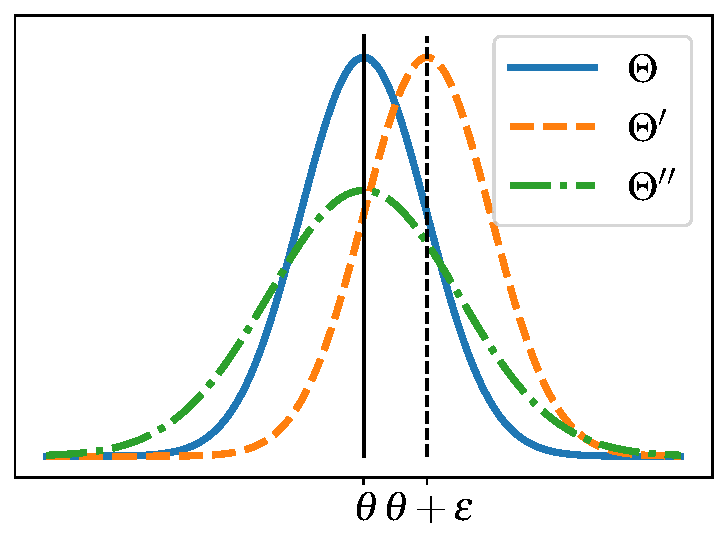
\includegraphics[width=0.5\textwidth]{figures/estimation/biais_variance}
  \caption{Distribution de 3 estimateurs de $\theta$.}
  \label{fig:biais_variance}
\end{figure}

\subsection{Exemple : Estimation non-biaisée de la variance}
\label{sec:unbiased_variance_estimation}
Considérons $X$ est de carré intégrable ($X \in \Lcal^2$), d'espérance $m$ et
de variance $\sigma^2$.

La \textbf{variance empirique} de $X$ est une variable aléatoire $S_n$, définie
par
\begin{equation}
  S_n = \frac1n \sum_{i=1}^n (X_i - M_n)^2,
  \label{eq:variance_empirique}
\end{equation}
où $M_n$ est la moyenne empirique telle que définie précédemment.

$S_n$ est un estimateur de $\sigma^2.$

Cependant, son biais vaut $\frac{-1}{n} \sigma^2$  (voir calcul
  section~\ref{sec:biais_variance_empirique}).

On propose donc la \textbf{variance empirique corrigée,} définie par 
\begin{equation}
  S^*_n = \frac1{n-1} \sum_{i=1}^n (X_i - M_n)^2,
  \label{eq:variance_empirique_corrigee}
\end{equation}
et qui est non-biaisée.

Néanmoins, le biais de la variance empirique tend vers 0 lorsque $n$ tend vers
$+\infty$. On parle alors d'un estimateur \textbf{asymptotiquement non-biaisé.}

\subsection{Précision d'un estimateur}
\label{sec:precision_estimateur}

Reprenons la figure~\ref{fig:biais_variance}. Les deux estimateurs $\Theta$ et
$\Theta^{\prime\prime}$ sont non-biaisés. Cependant, $\Theta^{\prime\prime}$ a
une plus grande variance ; une de ses réalisation a une probabilité plus grande
que pour $\Theta$ d'être éloignée de $\theta$. Ainsi, $\Theta^{\prime\prime}$
est \textit{moins précis} que $\Theta.$
  
Un estimateur non-biaisé sera considéré d'autant plus précis que sa variance
est faible.  Dans le cas général d'un estimateur biaisé, il faut aussi prendre
en compte le biais dans la définition de la précision. Un estimateur biaisé
mais de variance faible pourra donner de meilleures estimations (c'est-à-dire
plus proches de la vraie valeur) qu'un estimateur moins biaisé mais avec une
plus grande variance.

C'est pourquoi on utilise pour quantifier la précision d'un estimateur ponctuel
générique son \textit{erreur quadratique moyenne,} définie comme
\begin{equation}
  \text{EQM}(\Theta_n) = \EE((\Theta_n - \theta)^2) = \VV(\Theta_n - \theta) + \EE((\Theta_n - \theta))^2
  = \VV(\Theta_n) + \text{B}(\Theta_n)^2.
  \label{eq:eqm}
\end{equation}
Un estimateur sera ainsi d'autant plus précis que son erreur quadratique moyenne est faible.

\paragraph{Compromis biais-variance} Il est tout à fait possible qu'un
estimateur biaisé ait une meilleure précision qu'un estimateur non-biaisé, si
ce dernier a une plus grande variance !

\begin{figure}[h]
  \centering
  \begin{subfigure}[t]{0.4\textwidth}
    \centering
    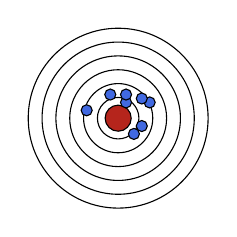
\begin{tikzpicture}
      \node[circle, minimum size=2, draw, fill=BrickRed] at (0, 0) {};
      \node[circle, minimum size=15, draw] at (0, 0) {};
      \node[circle, minimum size=25, draw] at (0, 0) {};
      \node[circle, minimum size=35, draw] at (0, 0) {};
      \node[circle, minimum size=45, draw] at (0, 0) {};
      \node[circle, minimum size=55, draw] at (0, 0) {};
      \node[circle, minimum size=65, draw] at (0, 0) {};

       \draw[fill=RoyalBlue] (0.4, 0.2) circle (2pt);
       \draw[fill=RoyalBlue] (-0.1, 0.3) circle (2pt);
       \draw[fill=RoyalBlue] (0.1, 0.2) circle (2pt);
       \draw[fill=RoyalBlue] (0.3, -0.1) circle (2pt);
       \draw[fill=RoyalBlue] (0.2, -0.2) circle (2pt);
       \draw[fill=RoyalBlue] (-0.4, 0.1) circle (2pt);
       \draw[fill=RoyalBlue] (0.1, 0.3) circle (2pt);
       \draw[fill=RoyalBlue] (0.3, 0.25) circle (2pt);
    \end{tikzpicture}     
    \caption{Biais faible, variance faible}
  \end{subfigure} \hfill
  \begin{subfigure}[t]{0.4\textwidth}
    \centering
    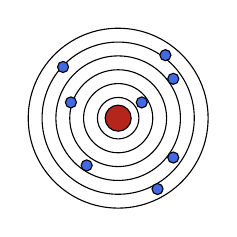
\begin{tikzpicture}
      \node[circle, minimum size=2, draw, fill=BrickRed] at (0, 0) {};
      \node[circle, minimum size=15, draw] at (0, 0) {};
      \node[circle, minimum size=25, draw] at (0, 0) {};
      \node[circle, minimum size=35, draw] at (0, 0) {};
      \node[circle, minimum size=45, draw] at (0, 0) {};
      \node[circle, minimum size=55, draw] at (0, 0) {};
      \node[circle, minimum size=65, draw] at (0, 0) {};

      \draw[fill=RoyalBlue] (0.6, 0.8) circle (2pt);
      \draw[fill=RoyalBlue] (-0.7, 0.65) circle (2pt);
      \draw[fill=RoyalBlue] (-0.4, -0.6) circle (2pt);
      \draw[fill=RoyalBlue] (0.5, -0.9) circle (2pt);
      \draw[fill=RoyalBlue] (0.7, -0.5) circle (2pt);
      \draw[fill=RoyalBlue] (-0.6, 0.2) circle (2pt);
      \draw[fill=RoyalBlue] (0.3, 0.2) circle (2pt);
      \draw[fill=RoyalBlue] (0.7, 0.5) circle (2pt);
    \end{tikzpicture}
    \caption{Biais faible, variance élevée}
  \end{subfigure}
  \begin{subfigure}[t]{0.4\textwidth}
    \centering
    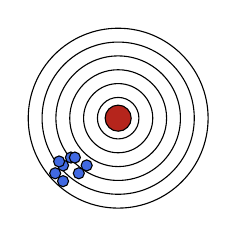
\begin{tikzpicture}
      \node[circle, minimum size=2, draw, fill=BrickRed] at (0, 0) {};
      \node[circle, minimum size=15, draw] at (0, 0) {};
      \node[circle, minimum size=25, draw] at (0, 0) {};
      \node[circle, minimum size=35, draw] at (0, 0) {};
      \node[circle, minimum size=45, draw] at (0, 0) {};
      \node[circle, minimum size=55, draw] at (0, 0) {};
      \node[circle, minimum size=65, draw] at (0, 0) {};

      \draw[fill=RoyalBlue] (-0.7, -0.6) circle (2pt);
      \draw[fill=RoyalBlue] (-0.6, -0.5) circle (2pt);
      \draw[fill=RoyalBlue] (-0.75, -0.55) circle (2pt);
      \draw[fill=RoyalBlue] (-0.5, -0.7) circle (2pt);
      \draw[fill=RoyalBlue] (-0.4, -0.6) circle (2pt);
      \draw[fill=RoyalBlue] (-0.8, -0.7) circle (2pt);
      \draw[fill=RoyalBlue] (-0.7, -0.8) circle (2pt);
      \draw[fill=RoyalBlue] (-0.55, -0.5) circle (2pt);
     \end{tikzpicture}
    \caption{Biais élevé, variance faible}
  \end{subfigure} \hfill
  \begin{subfigure}[t]{0.4\textwidth}
    \centering
    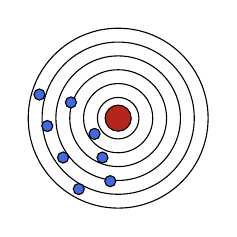
\begin{tikzpicture}
      \node[circle, minimum size=2, draw, fill=BrickRed] at (0, 0) {};
      \node[circle, minimum size=15, draw] at (0, 0) {};
      \node[circle, minimum size=25, draw] at (0, 0) {};
      \node[circle, minimum size=35, draw] at (0, 0) {};
      \node[circle, minimum size=45, draw] at (0, 0) {};
      \node[circle, minimum size=55, draw] at (0, 0) {};
      \node[circle, minimum size=65, draw] at (0, 0) {};

      \draw[fill=RoyalBlue] (-0.2, -0.5) circle (2pt);
      \draw[fill=RoyalBlue] (-1., 0.3) circle (2pt);
      \draw[fill=RoyalBlue] (-0.1, -0.8) circle (2pt);
      \draw[fill=RoyalBlue] (-0.5, -0.9) circle (2pt);
      \draw[fill=RoyalBlue] (-0.9, -0.1) circle (2pt);
      \draw[fill=RoyalBlue] (-0.6, 0.2) circle (2pt);
      \draw[fill=RoyalBlue] (-0.3, -0.2) circle (2pt);
      \draw[fill=RoyalBlue] (-0.7, -0.5) circle (2pt);
    \end{tikzpicture}
    \caption{Biais élevé, variance élevée}
  \end{subfigure}
  \caption{Illustration des concepts de biais et de variance par analogie avec
    un jeu de fléchettes. La quantité à estimer est le centre de la cible ; les
    fléchettes sont les estimations. Chacune des sous-figures présente un
    estimateur différent.}
  \label{fig:flechettes}
\end{figure}


\subsection{Convergence d'un estimateur $\bullet$}
\label{sec:convergence_estimateur}
On souhaite aussi d'un estimateur qu'il permette de s'approcher d'autant mieux
de la quantité qu'il estime que la taille de l'échantillon est grande. On parle
ici de la convergence d'une série de variables aléatoires réelles,
$(\Theta_n)_{n \in \NN^*},$ vers une valeur réelle, $\theta$ ; il s'agit donc
en fait de considérer la convergence vers une variable aléatoire $\Theta$ qui
vaut $\theta$ presque partout.

On dit que l'estimateur $\Theta_n$ de $\theta$ \textbf{est convergent} s'il
converge en probabilité vers $\theta:$
\begin{equation}
  \label{eq:estimateur_convergent}
  (\Theta_n)_{n \in \NN^*} \cvproba \theta.
\end{equation}

Si de plus la convergence est presque sûre,
$(\Theta_n)_{n \in \NN^*} \cvps \theta,$ on dit alors que $\Theta_n$ est un
estimateur \textbf{fortement convergent} de $\theta$.

\paragraph{Proposition} Un estimateur sans biais et de variance
asymptotiquement nulle est convergent.

\paragraph{Preuve} La preuve en a été faite dans l'exercice « Convergence vers
une constante » de Probabilité IV. Pour rappel, posons $\Theta_n$ un estimateur
non biaisé et de variance asymptotiquement nulle de $\theta \in \RR$,
c'est-à-dire que $\EE(\Theta_n) = \theta$ et $\VV(\Theta_n) \cvn 0.$ $\Theta_n$
est donc d'espérance et de variance bornées et ainsi dans $\Lcal^2.$ Enfin,
$  \EE((\Theta_n - \theta)^2) = \VV(\Theta_n) + B(\Theta_n)^2,$
et donc $\EE((\Theta_n - \theta)^2) \cvn 0,$ ce qui signifie que
$\Theta_n \cvltwo \theta$ et donc $\Theta_n \cvproba \theta. \hfill \square$

\paragraph{Remarque} On utilise en anglais le terme de ``\textit{consistent}'',
ce qui conduit les francophones à parfois parler d'estimateur consistant plutôt
que convergent.

\subsection{Exercice (estimation de la moyenne)}
\label{sec:exo_proprietes}
Nous cherchons à déterminer le poids moyen des bébés à la naissance en
France. Pour cela, nous disposons d'un échantillon $(x_1, x_2, \dots, x_n)$ de
$n$ mesures obtenues dans plusieurs maternités à travers le pays.

Nous supposons que cet échantillon est une réalisation d'un échantillon
$(X_1, X_2, \dots, X_n)$ de variables aléatoire réelles indépendantes et
identiquement distribuées, d'espérance $m$ et de variance $\sigma^2$.

On propose deux estimateurs de $m$ : 
\[
  M_n = \frac1n \sum_{i=1}^n X_i \text{ et } Z_n = \frac12 (X_n + X_{n-1}).
\]

Montrer que $M_n$ et $Z_n$ sont sans biais. Lequel choisir pour approcher $m$ ?

(Solution : section~\ref{sec:sol_proprietes}.)


%-*- coding: utf-8 -*-
\section{QCM}

\paragraph{Question 1.} Soit $X$ une variable aléatoire réelle suivant une loi
de Poisson de paramètre $\lambda$. Étant donné un échantillon aléatoire
$(X_1, X_2, \dots, X_n)$ de $X$, et une de ses réalisations
$(x_1, x_2, \dots, x_n)$, cocher le(s) estimateur(s) non biaisé(s) de $\lambda$
parmi les propositions ci-dessous :
\begin{itemize}
\item[$\square$] $L_1 = \frac1n \sum_{i=1}^n x_i.$
\item[$\square$] $L_2 = \frac1n \sum_{i=1}^n X_i.$
\item[$\square$] $L_3 = \frac1n \sum_{i=1}^n \left( X_i^2 - \left( \frac1n \sum_{j=1}^n X_j \right)^2 \right).$
\item[$\square$] $L_4 = \frac1n \sum_{i=1}^n \left( x_i^2 - \left( \frac1n \sum_{j=1}^n x_j \right)^2 \right).$
\end{itemize}


\paragraph{Indice.}
{%
\noindent
\rotatebox[origin=c]{180}{%
\noindent
\begin{minipage}[t]{\linewidth}
Quelles sont l'espérance et la variance d'une loi de Poisson de paramètre $\lambda$ ?
\end{minipage}%
}%

\paragraph{Question 2.} Un estimateur biaisé peut être plus précis qu'un estimateur non-biaisé.
\begin{itemize}
\item[$\square$] Vrai.
\item[$\square$] Faux.
\end{itemize}


\section*{Solution}
{%
\noindent
\rotatebox[origin=c]{180}{%
\noindent
\begin{minipage}[t]{\linewidth}
\paragraph{Question 1.} Il y a ici tout d'abord une question de vocabulaire :
un estimateur est une variable aléatoire, tandis qu'une estimation est sa
réalisation. Ainsi nous ne considérons que les formules avec $X$ et non pas
avec $x$.

On rappelle que $\EE(X) = \lambda$ et $\VV(X) = \lambda.$

Seul $L_2$ est un estimateur sans biais de $\EE(X) = \lambda$ : c'est la moyenne
empirique de $X$.

On peut refaire le calcul : les $X_i$ étant i.i.d. de même loi que $X,$ 
\[
  \text{B}(L_2) = \EE(L_2) - \lambda = \frac1n \sum_{i=1}^n \EE(X_i) - \lambda = 0.
\]

$L_3$ est la variance empirique de $X$ et $L_3$ est donc un estimateur
biaisé de $\VV(X) = \lambda$. \newline

\paragraph{Question 2.} Vrai. C'est le concept du compromis biais-variance
(cf. section~\ref{sec:precision_estimateur}).
\end{minipage}%
}%

%%% Local Variables:
%%% mode: latex
%%% TeX-master: "../../sdd_2025_poly"
%%% End:




\section{Estimation par maximum de vraisemblance}
Nous considérons toujours dans cette section un échantillon aléatoire
$(X_1, X_2, \dots, X_n)$ de taille $n \in \NN^*$ d'une variable aléatoire
réelle $X$, et une quantité $\theta \in \Scal \subseteq \RR$ à estimer. Nous
notons $\PP_X$ la loi de $X$.

Nous venons de voir comment caractériser un estimateur $\Theta_n$ afin de
choisir le meilleur estimateur parmi plusieurs. Mais comment \textit{proposer} un
estimateur de $\theta$ ?

Supposons que $(x_1, x_2, \dots, x_n)$ est une réalisation de
$(X_1, X_2, \dots, X_n)$. La technique que nous allons voir consiste à
maximiser la vraisemblance de l'échantillon, autrement dit la probabilité
d'observer cet échantillon étant donnée la valeur estimée de $\theta$.

\begin{exemple}
  Nous nous intéressons à la réussite d'élèves au baccalauréat en
  \^Ile-de-France, et disposons d'observations issues de plusieurs lycées de la
  région.

  Nous modélisons l'observation \og réussite \fg~ou \og échec \fg~comme la
  réalisation d'une variable aléatoire $X$, de domaine $E = \{0, 1\}$ ($0$
  correspondant à \og échec \fg~et $1$ à \og réussite \fg), et suivant une loi
  de probabilité $\PP_X$.  Un choix classique pour cette loi de probabilité est
  d'utiliser une loi de Bernoulli de paramètre $p$,:
  \[
    \PP_X(X=x) = p^x (1-p)^{1-x}.
  \] 
  Nos observations constituent un échantillon
  $(x_1, x_2, \dots, x_n)$, qui est une réalisation de l'échantillon aléatoire
  $(X_1, X_2, \dots, X_n)$ de composantes indépendantes et identiquement
  distribuées de même loi que $X$.

  Nous cherchons à estimer $p$ à partir de cet échantillon. 

  Supposons que notre échantillon contient $n=500$ élèves, dont $b=450$ ont
  eu le bac.

  La valeur $p=50\%$ est peu vraisemblable ; la valeur $p=90\%$ l'est beaucoup
  plus. C'est cette notion que nous allons formaliser par la suite.
\end{exemple}

La \textbf{vraisemblance} de l'échantillon $(x_1, x_2, \dots, x_n)$ quantifie à
quel point il est plausible d'observer cet échantillon en fonction de la valeur
de la quantité à estimer.

Pour tout $t \in \Scal$, nous notons $\PP_{X; t}$ la loi de $X$ paramétrée par
$t.$ Supposons qu'il existe une mesure $\mu$ sur $(\RR, \Bcal(\RR))$ telle que
$\PP_{X; t}$ s'écrive sous la forme $\PP_{X; t}= f_t \mu,$ où
$f_t: \RR \mapsto \RR_+$ est $\mu$-mesurable. Dans le cas où $X$ est discrète,
$\mu$ est la mesure de comptage et $f_t$ la fonction de masse de $X$. Dans le
cas où $X$ est à densité, $\mu$ est la mesure de Lebesgue et $f_t$ est la
densité de $X$. (Voir par exemple la section « Probabilités -- cadre général »
de Probabilités III.) La vraisemblance de $(x_1, x_2, \dots, x_n)$ est alors la
fonction de $t$ définie par
\begin{equation}
  L(x_1, x_2, \dots, x_n; t) = \prod_{i=1}^n f_t(x_i).
  \label{eq:likelihood}
\end{equation}

Notez que la loi de l'échantillon aléatoire $(X_1, X_2, \dots, X_n)$ est 
$  \PP_{X_1, X_2, \dots, X_n ; t} = \prod_{i=1}^n \PP_{X; t} $
car les $X_i$ sont indépendantes et identiquement distribuées.

On appelle alors \textbf{estimation par maximum de vraisemblance} ({\it maximum
  likelihood estimate} ou {\it MLE} en anglais) de $\theta$ une valeur
$\hatmle{\theta}$ qui maximise la vraisemblance de l'échantillon
$(x_1, x_2, \dots, x_n)$:
\begin{equation}
  \label{eq:mle_estimator}
  \hatmle{\theta} \in \argmax_{t \in \Scal} \prod_{i=1}^n f_t(x_i).
\end{equation}

\textbf{Un estimateur par maximum de vraisemblance} de $\theta$ est une
variable aléatoire réelle $\hatmle{\Theta}$ dont la valeur quand
$X_1=x_1, X_2=x_2, \dots, X_n=x_n$ est donnée par $\hatmle{\theta}$.

Pour simplifier les calculs, on choisira souvent de maximiser non pas
directement la vraisemblance mais son logarithme :
\begin{equation}
  \label{eq:lmle_estimator} 
  \hatmle{\theta} \in \argmax_{t \in \Scal}\sum_{i=1}^n \ln f_t(x_i).
\end{equation}

\begin{exemple}
  Reprenons notre exemple de réussite au baccalauréat.
  
  L'estimation par maximum de vraisemblance de $p$ est
  \begin{align*}
    \hatmle{p} & = \argmax_{t \in [0, 1]} \sum_{i=1}^n \ln \PP_{X; t}(X=x_i)
                          = \argmax_{t \in [0, 1]} \sum_{i=1}^n \ln 
                          \left( t^{x_i} (1-t)^{1-x_i}  \right) \\
                        & = \argmax_{t \in [0, 1]} \sum_{i=1}^n x_i \ln t + 
                          \left( n - \sum_{i=1}^n x_i \right) \ln (1-t).
  \end{align*}
  La fonction que nous cherchons à minimiser est
  $\ell: t \mapsto \sum_{i=1}^n x_i \ln t + \left( n - \sum_{i=1}^n x_i \right)
  \ln (1-t).$

  Rappelons que l'on note $b = \sum_{i=1}^n x_i.$ Si $b=n$, alors
  $\ell(t) = n \ln t$ et $\ell$ est maximale quand $t=1.$

  Si $b=0$, alors $\ell(t) = n \ln (1-t)$ et $\ell$ est maximale quand $t=0.$

  Enfin, si $0 < b < n,$ la fonction que nous cherchons à minimiser est
  concave, nous pouvons donc la maximiser en annulant sa dérivée :
  \begin{equation*}
    \frac{d \ell}{d t} = \sum_{i=1}^n x_i \frac1t - 
    \left( n - \sum_{i=1}^n x_i \right) \frac1{1-t},
  \end{equation*}
  ce qui nous donne
  \begin{equation*}
    (1 - \hatmle{p}) \left( \sum_{i=1}^n x_i \right) - \hatmle{p} \left( n - 
      \sum_{i=1}^n x_i \right) = 0
  \end{equation*}
  et donc, pour toutes les valeurs possibles de $b,$
  \begin{equation}
    \label{eq:mle_bernoulli}
    \hatmle{p} = \frac{1}{n} \sum_{i=1}^n x_i = \frac{b}{n}.
  \end{equation}
  
  L'estimateur par maximum de vraisemblance de $p$ est ainsi tout simplement la
  moyenne empirique de l'échantillon. Dans notre exemple, $p=450/500=90\%.$
\end{exemple}


\paragraph{Propriété $\bullet$} L'estimateur par maximum de vraisemblance est
(sous des hypothèses généralement vérifiées) convergent. La démonstration,
plutôt pénible, repose sur l'application de la loi des grands nombres : le
paramètre maximisant la vraisemblance maximise aussi la log-vraisemblance ainsi
que la log-vraisemblance divisée par $n$.

\subsection{Exercice} 
\label{sec:rayleigh_exo}
Soit $X$ une variable aléatoire réelle dont la densité de probabilité est donnée par 
\[
  f(x; \sigma^2) = \frac{x}{\sigma^2} \exp \left( - \frac{x^2}{2 \sigma^2} \right) \text{ pour } x \in [0, +\infty[.
\]
On pourra vérifier\footnote{Par exemple sur \href{https://fr.wikipedia.org/wiki/Loi_de_Rayleigh}{https://fr.wikipedia.org/wiki/Loi\_de\_Rayleigh}.} qu'il s'agit d'une loi de Rayleigh de paramètre d'échelle
$\lambda = \sqrt{2} \sigma$. Ainsi son espérance et sa variance sont données par 
\[
  \EE(X) = \sqrt{\frac{\pi}{2}} \sigma \text{\qquad et \qquad} \VV(X) =
  \frac{4-\pi}{2} \sigma^2.
\]
Donner l'estimateur par maximum de vraisemblance de $\sigma^2$.
Solution : voir section~\ref{sec:rayleigh_sol}.


\section{Estimation de Bayes $\bullet$}
\label{sec:bayes_est}
Supposons que plutôt que de ne pas connaître du tout la valeur du paramètre
$\theta$, nous ayons une bonne idée des valeurs qu'il peut prendre. Cette
information peut être très utile, surtout quand le nombre d'observations est
faible.

Pour en tirer parti, nous allons utiliser une variable aléatoire réelle
$\Theta$ à valeurs dans $\Scal$, dont la loi $\PP_{\Theta}$ est la \textbf{loi
  a priori}, c'est-à-dire définie avant d'avoir observé un échantillon. Il va
maintenant s'agir d'utiliser la formule de Bayes pour exprimer la \textbf{loi a
  posteriori}, c'est-à-dire conditionnellement à un échantillon aléatoire, de
$\Theta$.

Si $\Theta$ est discrète, la formule de Bayes nous permet
d'écrire la loi de $\Theta|X_1, X_2, \dots, X_n :$
\begin{equation}
  \label{eq:bayes_discret}
  \PP_{\Theta|X_1, X_2, \dots, X_n}(\Theta=t) = \frac{\PP_{\Theta}(t) \prod_{i=1}^n f_t(x_i)}{
    \sum_{u \in \Scal} \PP_{\Theta}(u) \prod_{i=1}^n f_u(x_i)}
\end{equation}

Si $\Theta$ est à densité, de densité $g_{\Theta},$ alors
$\Theta|X_1, X_2, \dots, X_n$ est aussi à densité et la formule de Bayes nous
permet d'écrire sa densité comme : 
\begin{equation}
  \label{eq:bayes_densite}
  g_{\Theta|X_1, X_2, \dots, X_n}(t) = \frac{g_{\Theta}(t) \prod_{i=1}^n f_t(x_i)}{
    \int_{\Scal} g_{\Theta}(u) \prod_{i=1}^n f_u(x_i) du}
\end{equation}
Ces manipulations de Bayes sont analogues à celles effectuées dans le poly de
Probabilités III, en particulier dans la section « Formule de balayage
conditionnel » et dans l'exercice « Loi conjuguées ».

En d'autres termes, l'observation d'un échantillon permet d'ajuster la loi a
priori de $\Theta$ en sa loi a posteriori. Cette idée est au c\oe{}ur
de \textbf{l'inférence bayésienne.}

\subsection{Estimation par maximum a posteriori}

L'\textit{estimation par maximum a posteriori} de $\theta$ est définie comme
une valeur de $\Scal$ qui maximise la loi a posteriori de $\Theta$. Ainsi dans
le cas discret,
\begin{equation}
  \label{eq:map_discret}
  \hatmap{\theta} \in \argmax_{t \in \Scal} \PP_{\Theta|X_1, X_2, \dots, X_n}(\Theta=t)
\end{equation}
et dans le cas à densité,
\begin{equation}
  \label{eq:map_densite}
  \hatmap{\theta} \in \argmax_{t \in \Scal} g_{\Theta|X_1, X_2, \dots, X_n}(t).
\end{equation}
   
L'estimateur par maximum a posteriori coincide avec l'estimateur par
maximum de vraisemblance si la distribution a priori utilisée est une
distribution uniforme.
  

\subsection{Estimation de Bayes}
L'estimation par maximum a posteriori est limitée dans le cas où la
distribution a postériori est multi-modale ; en effet, le mode le plus grand
peut être difficile à identifier par des algorithmes de gradient. De plus, elle
ne prend en compte qu'un seul point de la distribution a posteriori, plutôt que
de la considérer dans son intégralité.

L'estimation de Bayes de $\theta$ est définie comme une valeur de $\Scal$ qui
% est la mieux estimée par la loi a posteriori de $\Theta$
minimise en espérance une fonction de coût sur la loi a posteriori de $\Theta$.
Cette définition est
générale, et dépend de la fonction de coût utilisée. %du sens donné à « mieux estimée par » ;
Nous utiliserons
une des définitions les plus courantes, et considérons à partir de maintenant
l'erreur quadratique moyenne (définie section~\ref{sec:precision_estimateur}). 

L'\textbf{estimation de Bayes pour l'erreur quadratique moyenne} de $\theta$
est ainsi définie par
\begin{equation}
  \label{eq:bayes_estimator}
  \hatbys{\theta} \in \argmin_{t \in \Scal} \EE([(\Theta|X_1=x_1, X_2=x_2, \dots, X_n=x_n) - t)]^2).
\end{equation}


\paragraph{Propriété} L'estimation de Bayes pour l'erreur quadratique moyenne
est l'espérance de la distribution a posteriori de $\Theta$ : 
\begin{equation}
  \label{eq:bayes_estimator2}
  \hatbys{\theta}  = \EE(\Theta|X_1 = x_1, X_2=x_2, \dots, X_n=x_n).
\end{equation}

\paragraph{Preuve}
En effet, posons $t \in \Scal.$ Notons
$W = (\Theta|X_1=x_1, X_2=x_2, \dots, X_n=x_n)$ pour simplifier l'écriture.
Alors
\begin{equation*}
  \EE((W - t)^2) =  \EE(W^2) + t^2 - 2 t \EE(W) =  \EE(W^2) + [\EE(W) - t]^2 - \EE(W)^2.  
\end{equation*}
Comme ni $\EE(W^2)$ ni $\EE(W)^2$ ne dépendent de $t,$
$\hatbys{\theta}$ est obtenue en minimisant $(\EE(W) - t)^2$ et donc $\hatbys{\theta} = 
\EE(W). \hfill \square$

\begin{exemple}
  Reprenons notre exemple de taux de réussite au baccalauréat.  Nous supposons
  maintenant que $p$ est une réalisation d'une variable aléatoire $\Theta$ qui
  suit une loi bêta de paramètres $(\alpha, \beta)$
  (cf. section~\ref{sec:loi_beta}) et dont nous notons $g_\Theta$ la densité.

  Pour calculer l'estimateur de Bayes de $p$, il nous faut connaître la loi de
  $(\Theta|X_1=x_1, X_2=x_2, \dots, X_n=x_n)$. $\Theta$ étant à densité,
  $(\Theta|X_1=x_1, X_2=x_2, \dots, X_n=x_n)$ aussi et la loi de Bayes,
  combinée à l'hypothèse d'indépendance et de distribution identique des $X_i$,
  nous permet d'écrire sa densité comme 
  \begin{flalign*}
     & g_{\Theta|X_1=x_1, \dots, X_n=x_n}(t)  = \frac{\PP(X_1=x_1, \dots, X_n=x_n|\Theta=t) g_\Theta(t)}{\PP(X_1=x_1, \dots, X_n=x_n)} \\
    & = \frac{1}{\PP(X_1=x_1, \dots, X_n=x_n) B(\alpha, \beta)} 
    \prod_{i=1}^{n} t^{x_i} (1-t)^{1-x_i} t^{\alpha-1}
    (1-t)^{\beta-1} \\
    & = \frac{1}{\PP(X_1=x_1, \dots, X_n=x_n) B(\alpha, \beta)} 
    t^{b + \alpha - 1} (1-t)^{n - b + \beta - 1}. 
  \end{flalign*}
  
  On reconnaît ici la densité d'une nouvelle loi bêta.  Ainsi
  $(\Theta|X_1=x_1, \dots, X_n=x_n)$ suit une loi bêta de paramètres $(b + \alpha)$ et
  $(n - b + \beta).$

  L'estimation de Bayes de $p$ est ainsi
  \begin{equation*}
    \hatbys{p} = \EE(\Theta|X_1=x_1, X_2=x_2, \dots, X_n=x_n) = \frac{(b + \alpha)}{
      (b + \alpha) + (n - b + \beta)}
    = \frac{b + \alpha}{n + \alpha + \beta}.
  \end{equation*}
  Cette première égalité est obtenue d'après la formule donnant l'espérance
  d'une loi bêta (cf section~\ref{sec:loi_beta}).

  \textbf{Remarque importante}
  On peut réécrire cette estimation sous la forme
  \begin{equation*}
    \hatbys{p} = \frac{\alpha + \beta}{n + \alpha + \beta} \EE[\Theta] + 
    \frac{n}{n + \alpha + \beta} \hatmle{p}.
  \end{equation*}
  Ainsi, l'estimation de Bayes du paramètre $p$ est une combinaison linéaire de
  l'espérance de sa distribution a priori et de son estimation par maximum de
  vraisemblance.

  De plus, le coefficient multiplicatif de l'espérance a priori décroît en
  fonction de la taille $n$ de l'échantillon, tandis que le coefficient
  multiplicatif de l'estimation par maximum de vraisemblance croît en fonction
  de $n$. Ainsi, plus l'échantillon est grand, plus l'estimateur de Bayes fait
  confiance aux données, et s'éloigne de l'espérance a priori du paramètre,
  dont on est plus proche avec un petit échantillon.

  La figure~\ref{fig:bayes_estimate} illustre cet exemple.

  \textbf{Remarque} Le choix d'une loi bêta ne s'est pas fait au hasard. On
  retrouve ici les lois conjuguées présentées en exercice de Probabilités
  III. En inférence bayésienne, on dit qu'une loi a priori et une loi a
  posteriori sont conjuguées lorsqu'elles appartiennent à la même famille. En
  particulier, la loi bêta est conjuguée à elle-même pour une vraisemblance de
  Bernoulli.
\end{exemple}

\begin{figure}[h]
  \centering
  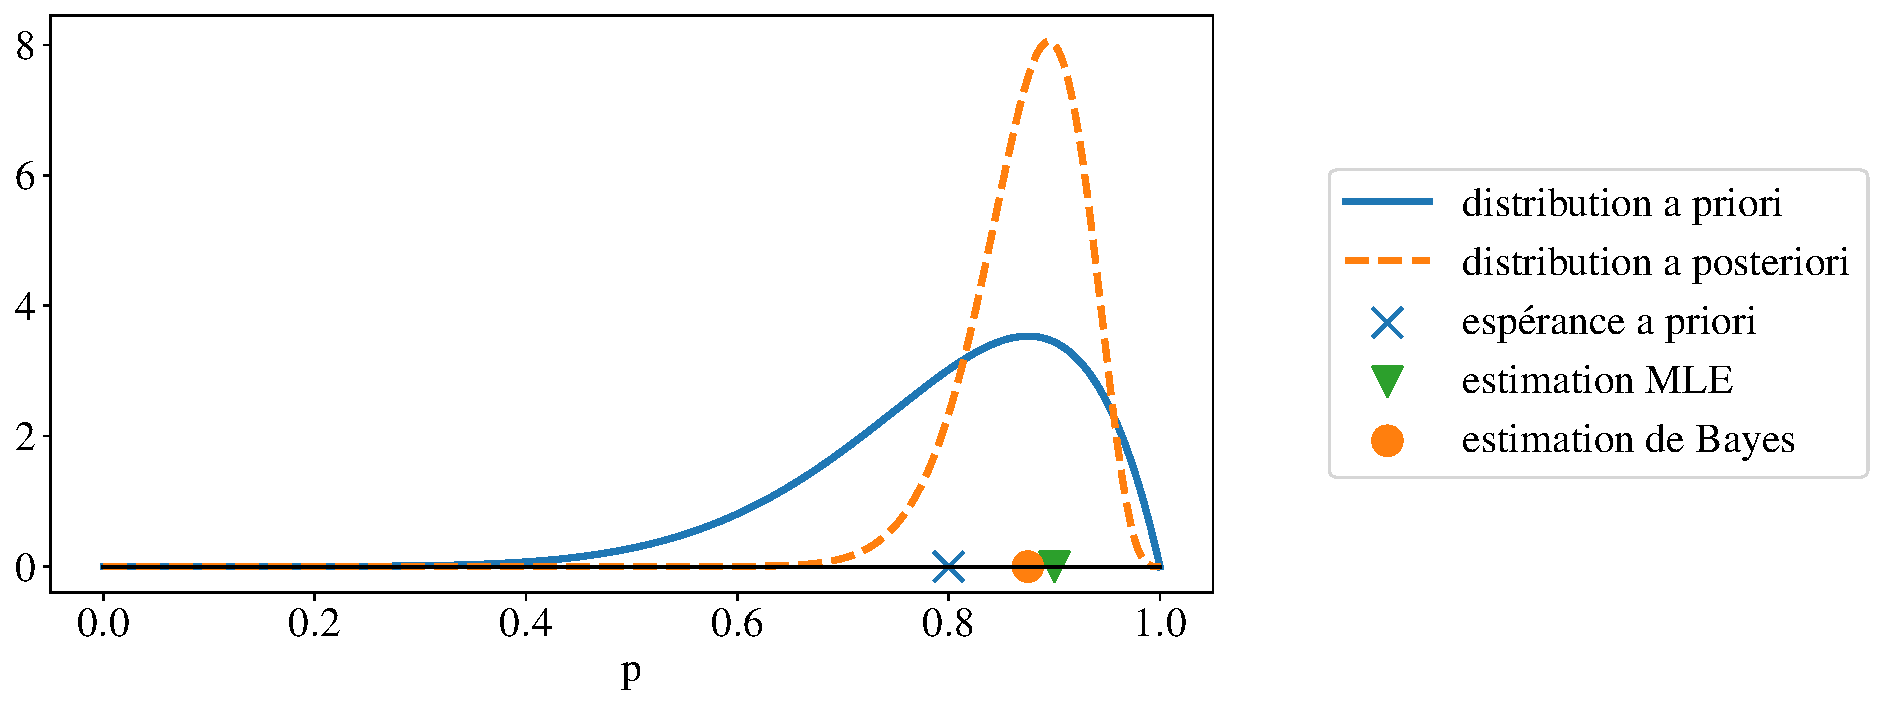
\includegraphics[width=\textwidth]{figures/estimation/bayes_estimate}
  \caption{Loi a priori et a posteriori pour le paramètre $p$ dans l'exemple du
    taux de réussite au baccalauréat. Sans voir de données, $p=0,80$,
    c'est-à-dire l'espérance de sa loi a priori (croix bleue). En utilisant
    uniquement l'échantillon, $p=0,90$, c'est-à-dire son estimation par maximum
    de vraisemblance (triangle vert). L'estimation de Bayes (rond orange) est
    intermédiaire.}
  \label{fig:bayes_estimate}
\end{figure}




\section{Compléments}
\subsection{Variance de la moyenne empirique} 
\label{sec:variance_moyenne_empirique}

Soit $X$ une variable aléatoire
réelle de carré intégrable, d'espérance $m$ et de variance $\sigma^2$. Soient
$X_1, X_2, \dots, X_n$ indépendantes et identiquement distribuées, de même loi
que $X$. 

Par définition de la variance, $\sigma^2 = \EE(X^2) - \EE(X)^2$ donc
$\EE(X^2) = \sigma^2 + m^2$.

Posons $M_n = \frac1n \sum_{i=1}^n X_i.$
\begin{align*}
  \VV(M_n) &= \EE(M_n^2) - \EE(M_n)^2 
   = \EE\left(\left(\frac1n \sum_{i=1}^n X_i\right)^2\right) - m^2 
   = \frac1{n^2} \EE\left( \sum_{i=1}^n X_i \sum_{j=1}^n X_j\right) - m^2 \\
  & = \frac1{n^2} \EE\left( \sum_{i=1}^n \left(X_i^2 + \sum_{j \neq i }^n X_i X_j \right) \right) - m^2 
   = \frac1{n} \left(\EE(X^2) + \sum_{j \neq i }^n \EE(X)^2 \right) - m^2, 
\end{align*}
par linéarité de l'espérance et car, pour $i \neq j$, $X_i$ et $X_j$ sont indépendantes et donc $\EE(X_iX_j) = \EE(X_i) \EE(X_j) = \EE(X)^2.$
Ainsi,
\[
  \VV(M_n) = \frac1{n} \left(\underbrace{\sigma^2 + m^2}_{\EE(X^2)} + (n-1) \, \underbrace{m^2}_{\EE(X)^2}  \right) - m^2 = \frac{\sigma^2}{n}.
\]

\subsection{Biais de la variance empirique} 
\label{sec:biais_variance_empirique}
Soit $X$ une variable aléatoire
réelle de carré intégrable, d'espérance $m$ et de variance $\sigma^2$. Soient
$X_1, X_2, \dots, X_n$ indépendantes et identiquement distribuées, de même loi
que $X$. 

Posons $M_n = \frac1n \sum_{i=1}^n X_i$ et $S_n = \frac1n \sum_{i=1}^n (X_i - M_n)^2.$ Alors
\begin{align*}
  \EE(S_n) = \frac1n \sum_{i=1}^n \EE((X_i - M_n)^2)  & =  
    \frac1n \sum_{i=1}^n \left( \EE(X_i^2) +  \EE(M_n^2) - 2 \EE(X_i M_n) \right)  \\
  & = \EE(X^2) + \EE(M_n^2) - \frac2n \sum_{i=1}^n \EE(X_i M_n).
\end{align*}
Nous avons montré lors du calcul de la variance de la moyenne empirique (section~\ref{sec:variance_moyenne_empirique}) que
$\EE(X^2) = \sigma^2 + m^2$ et que $\EE(M_n^2) = m^2 + \frac{\sigma^2}{n}.$
De plus, par linéarité de l'espérance,
\[
  \EE(M_n^2) = \EE\left( \left(\frac1n \sum_{i=1}^n X_i \right) M_n \right) = \frac1n \sum_{i=1}^n \EE(X_i M_n),
\]
et donc 
\[
  \EE(M_n^2) - \frac2n \sum_{i=1}^n \EE(X_i M_n) = - \EE(M_n^2).
\]

On obtient ainsi 
\[
  \EE(S_n) = (\sigma^2 + m^2) - \left(m^2 + \frac{\sigma^2}{n}\right) = \frac{n-1}{n} \sigma^2.
\]
La variance empirique est donc biaisée et son biais vaut 
\[
  \text{B}(S_n) = \EE(S_n) - \sigma^2 = - \frac1n \sigma^2.
\]

\subsection{Solution de l'exercice~\ref{sec:exo_proprietes}}
\label{sec:sol_proprietes}
La démonstration pour la moyenne empirique $M_n$ a été faite plus haut.

En ce qui concerne $Z_n$, 
\[
  \EE(Z_n) = \frac12 (\EE(X_n) + \EE(X_{n-1})) = m.
\]

Nous avons assez naturellement envie d'utiliser $M_n$, qui utilise toutes les
observations, plutôt que $Z_n$, qui n'en utilise que deux.

Pour nous en convaincre, nous pouvons comparer les variances de $M_n$ et
$Z_n$. La variance de la moyenne empirique est $\VV(M_n) = \frac{\sigma^2}{n}$
(voir plus haut). La variance de $Z_n$, elle, vaut
\[
  \VV(Z_n) = \frac14 \left( \VV(X_n) + \VV(X_{n-1}) \right) = \frac{\sigma^2}{2},
\]
la première égalité étant obtenue par indépendance de $X_n$ et $X_{n-1}$.

$Z_n$ est ainsi un estimateur bien moins précis que $M_n$ dès que $n>2.$

\subsection{Loi Beta}
\label{sec:loi_beta}
La densité de probabilité de la {\it loi bêta} de paramètres
$\alpha, \beta > 0$, définie sur $0 \leq u \leq 1$, est donnée par :
\begin{equation}
  \label{eq:beta_distribution}
  f_{\alpha, \beta} (u) = \frac{u^{\alpha -1} (1-u)^{\beta-1}}{B(\alpha, \beta)}     
\end{equation}
où
$B(\alpha, \beta) = \frac{\Gamma(\alpha) \Gamma(\beta)}{\Gamma(\alpha+\beta)}$
et $\Gamma$ est la fonction gamma. L'espérance de cette loi est
$\frac{\alpha}{\alpha + \beta}$.

\subsection{Solution de l'exercice~\ref{sec:rayleigh_exo}}
\label{sec:rayleigh_sol}
Soit $(x_1, x_2, \dots, x_n)$ un échantillon de $X$ de taille $n \in \NN^*.$ La
log-vraisemblance de l'échantillon est donnée par
\[
  \ell(x_1, x_2, \dots, x_n; \sigma^2) = \sum_{i=1}^n \ln \left(
    \frac{1}{\sigma^2} x_i \exp\left(- \frac{x_i^2}{2\sigma^2} \right)\right) 
  = -n \ln(\sigma^2) + \sum_{i=1}^n \ln(x_i) - \frac{1}{2\sigma^2} \sum_{i=1}^n x_i^2.
\]
Ainsi, l'estimation par maximum de vraisemblance de $\sigma^2$ est donnée par :
\[
  \hatmle{\sigma^2} \in \argmax_{s \in \RR_+} \left(-n \ln(s) + \sum_{i=1}^n \ln(x_i) - 
\frac{1}{2s} \sum_{i=1}^n x_i^2\right).
\]
On obtient un point critique de la fonction de $\RR_+$ dans $\RR$ qui à $s$
associe $-n \ln(s) + \sum_{i=1}^n \ln(x_i) - \frac{1}{2s} \sum_{i=1}^n x_i^2$
en annulant sa dérivée, qui vaut :
\[
  s \mapsto - \frac{n}{s} + \frac12 \sum_{i=1}^n x_i^2 \frac{1}{s^2},
\]
et donc 
\[
  \hatmle{\sigma^2} = \frac{1}{2n} \sum_{i=1}^n x_i^2.
\]
(On vérifiera que ce point critique est bien un maximum.)
Ainsi, étant donné un échantillon aléatoire $(X_1, X_2, \dots, X_n)$ de $X$,
l'estimateur par maximum de vraisemblance de $\sigma^2$ est donné par
\[
  S_n = \frac{1}{2n} \sum_{i=1}^n X_i^2.
\]


\begin{plusloin}
\item Un exercice sur la fonction de répartition empirique vous a été proposé
  dans le poly de Probabilité III.
\item On peut construire un estimateur par la \textit{méthode des moments}, qui
  consiste à faire coincider les moments théoriques de $\PP_X$ (qui dépendent
  donc de $\theta$) avec les moments empiriques de l'échantillon. La loi des
  grands nombres justifie en effet d'approcher la moyenne par la moyenne
  empirique. Cette méthode est généralement moins précise que le maximum de
  vraisemblance.
\item Plus la variance d'un estimateur est faible, plus cet estimateur
  peut-être considéré comme précis. La \textit{borne de Cramér-Rao} est une
  borne inférieure de cette variance pour un estimateur sans biais, en se
  basant sur l'information de Fisher. On dit qu'un estimateur est
  \textit{efficace} s'il est non-biaisé et que sa variance tend vers sa borne
  de Cramér-Rao.
\end{plusloin}

%\clearpage
%-*- coding: utf-8 -*-

\section{QCM}
\paragraph{Question 1.} Soit $(x_1, x_2, \dots, x_n)$ un échantillon d'une
variable aléatoire $X$ discrète. On suppose que $X$ suit une loi paramétrisée
par $\gamma$. La vraisemblance de $(x_1, x_2, \dots, x_n)$ est donnée par
\begin{itemize}
\item[$\square$] $\PP(X=x_1, X=x_2, \dots, X=x_n, \gamma)$
\item[$\square$] $\PP(X=x_1, X=x_2, \dots, X=x_n | \gamma)$
\item[$\square$] $\PP(\gamma | X=x_1, X=x_2, \dots, X=x_n)$
\item[$\square$] $\prod_{i=1}^n \PP(X=x_i|\gamma)$
\item[$\square$] $\prod_{i=1}^n \PP(\gamma|X=x_i)$
\end{itemize}

\paragraph{Question 2.} Soit $X$ une loi exponentielle de paramètre
$\lambda$. L'estimateur par maximum de vraisemblance de $\lambda$ est donné par
\begin{itemize}
\item[$\square$] $L_n = n \ln(\lambda) - \lambda \sum_{i=1}^n X_i,$ où $(X_1, X_2, \dots, X_n)$ est un échantillon aléatoire de $X$
\item[$\square$] $\widehat{\lambda} = n \ln(\lambda) - \lambda \sum_{i=1}^n x_i,$ où $(x_1, x_2, \dots, x_n)$ est un échantillon aléatoire de $X$
\item[$\square$] $L_n = \frac{n}{\sum_{i=1}^n X_i},$ où $(X_1, X_2, \dots, X_n)$ est un échantillon aléatoire de $X$
\item[$\square$] $\widehat{\lambda} = \frac{n}{\sum_{i=1}^n x_i},$ où $(x_1, x_2, \dots, x_n)$ est un échantillon aléatoire de $X$.
\end{itemize}

\paragraph{Question 3. $\bullet$} L'estimateur de Bayes est plus proche de l'espérance a
priori que de l'estimateur par maximum de vraisemblance quand la taille de
l'échantillon est
\begin{itemize}
\item[$\square$] grande
\item[$\square$] petite
\item[$\square$] ça dépend.
\end{itemize}



\section*{Solution}

{%
\noindent
\rotatebox[origin=c]{180}{%
\noindent
\begin{minipage}[t]{\linewidth}
\paragraph{Question 1.} Par définition (cf. équation~\ref{eq:likelihood}),
\[
L(x_1, x_2, \dots, x_n; \gamma) = \PP(x_1, x_2, \dots, x_n | \gamma) = \prod_{i=1}^n \PP(x_i|\gamma).
\]

\paragraph{Question 2.} 
Par définition la vraisemblance d'un échantillon $(x_1, x_2, \dots, x_n)$ est donnée par
\[
  L(x_1, x_2, \dots, x_n; \lambda) = \prod_{i=1}^n \lambda e^{- \lambda x_i}
  = \lambda^n \prod_{i=1}^n e^{- \lambda x_i},
\] 
et donc sa \textit{log-vraisemblance} vaut 
\[
  \ell(x_1, x_2, \dots, x_n; \lambda) = \ln \left(\lambda^n \prod_{i=1}^n e^{- \lambda x_i}\right)
  = n \ln(\lambda) - \lambda \sum_{i=1}^n x_i.
\]
La fonction $\lambda \mapsto n \ln(\lambda) - \lambda \sum_{i=1}^n x_i$ est
concave sur $]0, +\infty[ \rightarrow \RR$ et on peut donc la maximiser en
annulant sa dérivée.

On obtient \textit{l'estimation par maximum de vraisemblance} de $\lambda$ suivante :
\[
  \hatmle{\lambda} = \frac{n}{\sum_{i=1}^n x_i}
\]
et, si on appelle $(X_1, X_2, \dots, X_n)$ un échantillon aléatoire de $X$, on
obtient \textit{l'estimateur par maximum de vraisemblance} de $\lambda$ :
\[
  L_n = \frac{n}{\sum_{i=1}^n X_n}.
\]


\paragraph{Question 3.} La tendance que nous avons observée sur l'exemple de la
section~\ref{sec:bayes_est} (cf. « Remarque importante ») se vérifie en général : plus on
observe d'échantillons, plus on s'éloigne de l'a priori pour se rapprocher d'un
estimateur issu uniquement des données.
\end{minipage}%
}%

%%% Local Variables:
%%% mode: latex
%%% TeX-master: "../../sdd_2025_poly"
%%% End:




%%% Local Variables:
%%% mode: latex
%%% TeX-master: "../sdd_2025_poly"
%%% End:


